\include{__header__}

\begin{document}

\paragraph{О-01}
Какова интенсивность света в центре дифракционной картины от круглого экрана, если он закрывает всю первую зону Френеля? Интенсивность света в отсутствие экрана равна $I_0$.\\

\begin{wrapfigure}[12]{r}{0.4\linewidth}
	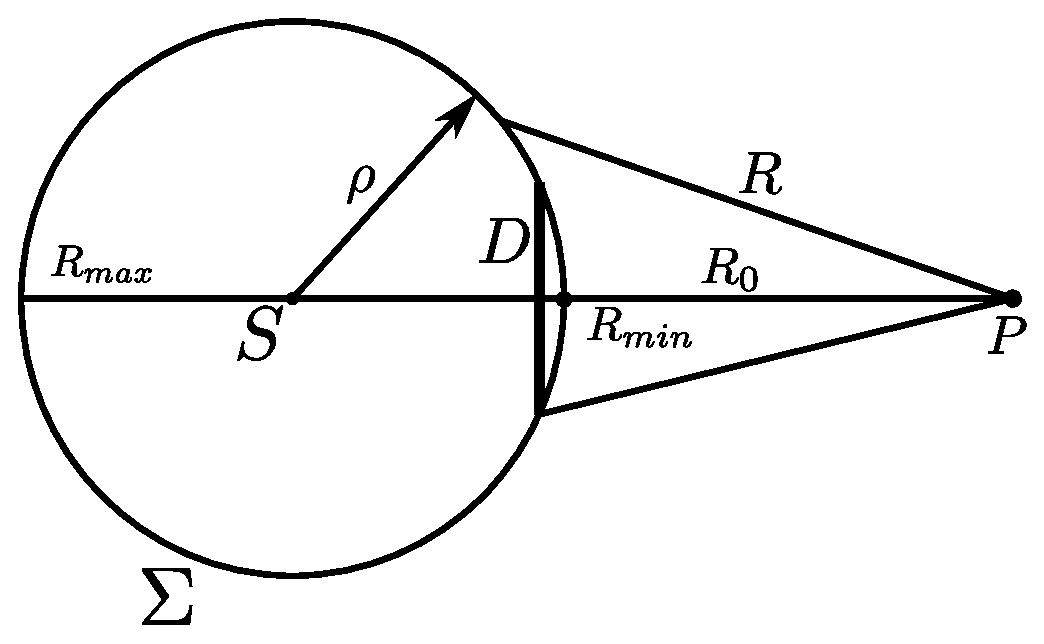
\includegraphics[width=1\linewidth]{img/o-01}
	\caption{Схема задачи}
	\label{o-01-diafrag}
\end{wrapfigure}

По формуле для напряженности электрического поля света, пропущенного через диафрагму радиуса $R_{max}$, и закрытой центральной областью радиуса $R_{max}$. (см. Рис. \ref{o-01-diafrag}) получим:
\begin{flalign}
\begin{split}
E &= E_0(K(R_{min})e^{ik(R_{min}-R_0)} - \\
  &- K(R_{max})e^{ik(R_{max}-R_0)}),
\end{split}
\label{o-01-formula}
\end{flalign}
где $K(R)$ - медленно монотонно убывающая функция такая, что $K(R_0) = 1$ и $K(R_0 + 2\rho) = 0$

Из того, что круглый экран закрывает первую зону Френеля получим 
$R_{max} = R_0 + 2\rho$, $\displaystyle R_{min} = R_0 + \frac{\lambda}{2}$, где $\lambda$ - длина волны света. Тогда $K(R_{max}) = 0$ и из (\ref{o-01-formula}):
\begin{flalign*}
&E = E_0K(R_0+\frac{\lambda}{2})e^{ik\lambda/2}
\Rightarrow (k = \frac{2\pi}{\lambda}) \\ \Rightarrow
&E = E_0K(R_0+\frac{\lambda}{2})e^{i\pi}
\Rightarrow (e^{i\pi} = -1, K(R_0 + \frac{\lambda}{2}) = K_1) \\ \Rightarrow
&E = -E_0K_1
\end{flalign*}
Тогда интенсивность света находится по формуле:
$$
I = E^2 \Rightarrow I = E_0^2K_1^2 = I_0K_1^2
$$
\end{document}